%% 
%% Copyright 2016 Icm Ltd
\documentclass[12pt,final,3p]{CSP}
\usepackage{amssymb}
\usepackage{changepage}
\usepackage[letterpaper,margin=0.75in]{geometry}
\usepackage{setspace}
\usepackage{amsmath}
  \usepackage{tikz}
    \usetikzlibrary{matrix}
\usepackage[ruled,vlined]{algorithm2e}
% \doublespacing


\begin{document}

\begin{frontmatter}
\setcounter{page}{1}
\title{Recusing Time and Energy Consumption in Wireless Networks using Edge Computing}

\author[mymainaddress]{Sepehr Sabour}

%\author[mysecondaryaddress]{Global Customer Service\corref{mycorrespondingauthor}}
%\cortext[mycorrespondingauthor]{Corresponding author}
%\ead{support@Icm.com}
\address[mymainaddress]{sepehr.sabour@ucalgary.ca}
\nocite{*}
\begin{abstract}\rm
\begin{adjustwidth}{2cm}{2cm}{\itshape\textbf{Abstract:}} 
Increasing the number of computing demand IoT applications, like security control, health check, and auto vehicles, in recent years leads us to use new computing structures. Edge computing, computing data using computers located on the edge of the communication network, has a myriad of benefits, including reducing time and energy consumption. In this architecture IoT devices can offload the collected data to an edge computer and save energy.

However, using edge processors in wireless networks is more challenging due to the fact that the number of devices in a wireless network is uncertain. For example, the number of smart vehicles that use edge processors in a district is random. Also, there are various applications with different requirements in the system.Sensors, like health control devices, need to use low battery power and applications like auto-driver are highly delay-sensitive. In result of randomness and heterogeneity of devices in this kind of network, and limited computing and network resources we need to find a suitable policy for offloading the tasks.

This project presents a policy for task offloading decision making and regulating transmission power of nodes. The simulation results of the method shows huge decrease in computing cost, and lead us to conclude the advantages of the proposed approach.

\end{adjustwidth}
\end{abstract}


\begin{keyword}\rm
\begin{adjustwidth}{2cm}{2cm}{\itshape\textbf{Keyword:}}  
Edge Computing, Wireless Network, Optimization 
\end{adjustwidth}
\end{keyword}

\end{frontmatter}

\section{Introduction}
\label{}
\noindent
Reducing computing costs has been an essential topic since the first days of introducing computers to people's lives. The cost of computation can be in different domains, including time, energy, money, etc. \textbf{But how can we compute tasks with lower costs? } Implementing fast and energy-efficient processors, algorithms optimization, and cloud computing are only a few examples of myriad answers that have been given to this question.  Nevertheless, introducing new applications makes scientists try to find more solutions for new computing problems.

We use Internet of Things applications every day in different aspects of our lives, such as smart homes, smart vehicles, and e-health applications. Two critical requirements of IoT applications are reducing processing delay and energy consumption. Short response time is essential for some applications like autonomous vehicles and e-Health. On the other hand, in some applications, we need to reduce consumed energy as much as possible. Due to the short battery lifetime of IoT sensors, this requirement is very crucial for most of the IoT applications. Studies on the IoT applications show us for different applications, these two requirements do not have the same importance.

In this project, we tried to reduce time and energy costs in computing. We consider a multi-objective problem to optimise resource allocation in a edge computing network. We propose edge computing for reducing the costs of IoT systems. Edge computing introduced by Cisco in 2012 \cite{Bonomi:2012:FCR:2342509.2342513}. The main idea of this method is using devices on the edge of networks for computing tasks. The benefits of using edge computing are including less computing time, saving energy, and efficient usage of network bandwidth. However, using edge computing is not always useful. In general offloading tasks to edge computing is a good chose if the other alternatives, local computing and cloud computing, spend more costs. Thus task offloading problem is one of the challenges in the edge computing area. 

Much research has been done in the field of edge computing offloading recently and still being done. Researchers have worked on finding the best offloading strategy to reduce the costs of computing. Minimizing power consumption or the latency of the system has remained the prime concern for the majority of researchers. However, there are just a few numbers of projects that consider both latency and energy consumption.

In \cite{8742650} and \cite{7553459} authors proposed offloading algorithm to reduce energy consumption in IoT networks. The mentioned algorithm in \cite{7553459}  focused on finding an optimum offloading vector. In \cite{8742650} authors also considered transmit covariance matrix and in physical layer of the network as a decision variable. In both cases the outputs are binary offloading policy. 

Decreasing time cost is studied in \cite{8314696} and \cite{7130662}. In both projects the proposed algorithm finds an optimal offloading vector.  \cite{7130662} also suggested a solution for finding energy-efficient CPU-cycle frequency. Another advantage of  \cite{7130662} is that partial offloading is considered in the method. 

There are few works like \cite{8234686} that focused on reducing cost of time and energy simultaneously. The proposed approach finds an optimum offloading vector and delay-energy tradeoff. In this method also does not offload tasks partially. 

The main contribution of this project is introducing a multi-objective optimization problem and finding an optimal solution for  offloading in edge computing systems to reduce total cost. Also in this project we find a best choice for computing and network resources such as \textbf{Transmission Power, CPU Frequency and Tramsimission Rate}

\section{System Model}
\noindent
In this section, we will introduce the system model studied in this report, i.e., an edge computing system with various applications. Then we discuss both time and energy models. 
\subsection{Edge Computing System with Various Applications}
\noindent
In this project, we consider a wireless network of different devices and applications. The set of devices in this network consists of a set of users equipment (UE) and one edge computer. $I$ is the set of UEs in the network. Each UE has one and only one computing task at each time. Different tasks in the network have different quality of service requirements. 
% $\alpha$ is the weight of energy consumption, and $\beta$ is the weight of latency for node $i$. These two parameters should satisfy the following conditions: $1 \geq \alpha,\beta \geq 0$ and $\alpha + \beta = 1$ . Also, the priority of each task can be different than other ones. $w_i$ is the priority of node $i$ and $w_i > 0$.

We assume code-division multiple access (CDMA) as the multiple access method of the uplink. It means devices send data using same time and frequency resources. Since using in code division approach, the transmission signal of unintended transmitters can cause interference on receivers. Thus the amount of Signal-to-interference-plus-noise ratio (SINR) per each node should be higher than a threshold.  SINR for each node is given by:
\begin{equation}
    SINR_i =  \frac{p_i d_i^{-\alpha}}{\sum_{\forall j \in I, j \neq i } p_j d_j^{-\alpha} + N} \hspace{10} \forall i \in I
\end{equation}
Where $p_i$ is the power level of node $i$ and $N$ is background noise power.  $\alpha$ and $d_i$ are channel gain function of the link and distance between node i and the edge computer, respectively.
Also, the amount of SINR should satisfy the following operation constraint, where $\theta$ is the minimum required SINR for a successful transmission.
\begin{equation}
    SINR_i \geq \theta \hspace{10}  \forall i \in I
\end{equation}
As mentioned in the introduction section, the studied offloading problem in this project is a Binary offloading problem, and we cannot submit task partially. For this manner, variable $x_i$ is introduced here. $x_i$ shows that whether task $i$ should offload to the edge computer or not.  Therefore $x_i = 1$ means offloading the whole task to edge computing, and $x_i = 0$ means using only the local computer for computing the task.
\subsection{Time Model}
The time that we need to compute a task is a maximum of spent time at the local computer and the edge computer. Hence we have:
\begin{equation}
     D_{i} = \max{(D^e_i,D^{l}_i)} \hspace{10} \forall i \in I
\end{equation}
Where $D^{l}$ and $D^{e}$ are computing delays at local and edge computers, respectively. The delay for edge computing can be expressed by following formula:
\begin{equation}
     D^e_i = D^{tr}_i + D^{ec}_i \hspace{10} \forall i \in I
\end{equation}
In this equation we present that a required time for executing a task in a edge computer consists of the time that we need to send data to the computer and processing time. Sending data, processing data at the edge and executing task locally be expressed by following formulas respectively:
\begin{equation}
      D^{tr} = (x_i d_i) / r_i\hspace{10} \forall i \in I
\end{equation}
\begin{equation}
      D_i^{ec} = \frac{c_i(1-x_i)}{f_{i,serv}}\hspace{10} \forall i \in I
\end{equation}

and the delay for executing tasks locally is given by:
\begin{equation}
      D_i^{l} = \frac{c_ix_i}{f_{i,l}}\hspace{10} \forall i \in I
\end{equation}
where $c_i$ is the number of bits for each task, and $d_i$ is the number of CPU cycles needed for executing the task. Also $r_i$ is transmission rate that can be calculated by:
\begin{equation}
      r_i \geq 2w\log{(1 +SINR_i)}\hspace{10} \forall i \in I
\end{equation}
\subsubsection{Energy Model}
\noindent

Total computing energy is the summation of consumed energy in the edge computer and the local device, which can be expressed by the following equation:

\begin{equation}
      E_i = E^l_i + E^e_i\hspace{10} \forall i \in I
\end{equation}

Where is the consumed energy in the edge computer and can be calculated by:
\begin{equation}
      E_i^e = p_iD_i^{tr}\hspace{10} \forall i \in I
\end{equation}
and the amount of energy spends by device for executing the task is given by:
\begin{equation}
      E^l_i = x_i\epsilon f^2_ic_i\hspace{10} \forall i \in I
\end{equation}
where $\epsilon$ is Effective switched capacitance of ...

\subsection{Problem Formulation}
In  this  section,  we  will  first  introduce  the  performance metric,  namely,  the  execution  cost.  The  execution  cost  minimization problem  will  then  be  formulated  and  its optimization challenges will be identified.
\noindent
\subsubsection{Execution Cost Minimization Problem}
Execution delay is one of the key measures for the QoS of the applications,  which  will  be  adopted  to  optimize  the computation offloading policy for the considered edge computing system. Also as mentioned before there are lots of applications that need to reduce the energy usage as much as possible. So the objective of the project is minimizing the cost of the task execution in term of time and energy. The objective is:

\begin{subequations}
\begin{alignat}{2}
A: &\!\min_{x,p,f_l,f_s}        &\qquad& \sum_{\forall i \in I} \omega_i (\alpha_iD_i + \beta_iE_i)&\\
&\text{s.t.} &      & 0 \leq x_i \leq 1& \forall i \in I \\
& &      & p_{min} \leq p_i \leq  p_{max} & \forall i \in I \\
& &      & \sum_{\forall i \in I} f_{i,ser} \leq f_{server} & \\
& &      & SINR_i \geq \theta & \forall i \in I \\
& &      & f_{i,l} \leq f_{max}& \forall i \in I  
\label{eq:main}
\end{alignat}
\end{subequations}

\subsubsection{Problem Analysis}
In the considered edge computing system state is composed assigned task to each UE, the computation offloading decision, including the scheduled edge and local computer CPU-cycle frequencies, the allocated transmit power and task partial offloading vector. The objective is the weighted aggregated execution cost. An increase in the transmit power level of a device can increase the interference over other devices. On the other hand, we have a limited amount of computing resources due to the limited capacity of CPUs. The more CPU power for a task we assign, the less executing time we need. Thus we need to allocate a suitable amount of CPU frequency to each task to minimize the cost. 

Local CPU frequently, edge CPU frequently, and task partial offloading vector are decision variables of the given problem. As we can see in problem $A$, the optimization problem is not linear, so we need to have some relaxation in solving it.

In the following section, we will propose a relaxation algorithm to solve problem $P$ , which enjoys the following favorable properties:

\begin{itemize}
    \item We need to find the right CPU frequency for the local computer. To satisfy the constraint (12f) the assigned frequency must be less than $f_{max}$.
    \item Also, we need to replace the edge CPU frequency variable with a constant value. This value should be selected base  on the priority of the task.
    \item For finding SINR, we have the transmission power variable as a denominator, so we need to change the variable to a constant variable. Hence we introduced an algorithm to find an optimum value for the power levels that satisfy constraints (12c) and (12e).
\end{itemize}

\subsubsection{Problem Relaxation}
First, we try to find an optimum transmission power level for each node. For this purpose, we introduce the following optimization problem:

\begin{subequations}
\begin{alignat}{2}
P: &\!\max &\qquad& \sum_{\forall i \in I} p_i&\\
&\text{s.t.} &      & p_{min} \leq p_i \leq p_{max}& \forall i \in I \\
& &      & SINR_{i} \geq \theta & \forall i \in I 
\label{eq:main}
\end{alignat}
\end{subequations}

This problem can also be expressed as a minimization problem:

\begin{subequations}
\begin{alignat}{2}
P^\prime: &\!\min &\qquad& \sum_{\forall i \in I} p_i&\\
&\text{s.t.} &      & p_{min} \leq p_i \leq p_{max}& \forall i \in I \\
& &      & SINR_{i} \geq \theta & \forall i \in I \\
& &      & r_{i} \geq R_{min} & \forall i \in I 
\label{eq:main}
\end{alignat}
\end{subequations}
Where $r_{i}$ is the data for node $i$ and $R_min$ is minimum data rate per each node. 

We should choose one of the algorithms according to the characteristics of the applications in the network. We showed that increasing a transmission power increases the consumed energy by the node but decreases the transmission delay and vice versa. Thus if the majority of the applications are delay-sensitive, we should use problem $P$ and if energy is the main concern in the network, problem $P^\prime$ would be the right choice.

By growing the number of nodes in the network eventually we cannot assign a power level more than minimum possible power to all the nodes. Hence some nodes should backoff form sending data. The algorithm 1 is a proposed approach for assigning power level to nodes.

 
\begin{algorithm}[H]
\SetAlgoLined
\KwResult{Power assignment vector}
 initialization\;
 Add all the nodes to set $S$\;
 \While{$S$ is not empty}{
  Solve problem $P$ and find optimum value for nodes in set $S$
  \eIf{There is a node in $S$ with assigned power less than minimum power}{
   Sort $S$ by descending priority order\;
   Pick the node with lowest priority\;
   Set node's power to zero\;
   Remove the node from $S$\;
   }{
   The optimum power assignment vector has been found\;
   Terminate algorithm\;
  }
 }
 \caption{Prioritized Power Assignment Algorithm}
\end{algorithm}


Since we have a limited amount of capacity in the edge processor, we split the resource based on the priority of each task. We could split the available frequency equally, but the proposed approach gives us a better result. In the section, we will compare the proposed method to the other alternative. For each task we calculate the CPU-cycle frequency by:

\begin{equation}
    f_{i,ser} = \frac{\omega_i \times f_{server}}{\sum_{\forall i \in I} \omega_{i}} \hspace{10} \forall i \in I
\end{equation}

For allocating the amount of CPU frequency of local computers, first, we assume that all the nodes use maximum available CPU frequency. 

\subsection{Numerical Results}
In this section, we evaluate the performance of our proposed our method through the montecarlo simulation. We consider there are $N$ nodes randomly distributed in a $100 * 100$ area.We have used poison point process method to generate the locations of the nodes. Also using poison random we selected QoS weights for each UI. Maximum and minimum transmit powers for devices in the network are $0.1$ and $0.001$ respectively. We considered a CPU with maximum CPU-cycle $5 GHz$ for edge computer and a CPU with maximum CPU-cycle $400 MHz$ for processors in UEs. In the simulated network the maximum bandwidth is $10 MHz$, SINR threshold is $10^-26$ and background noise power is $10^13 W$. 
For computing tasks in the network we granted random priorities and same data sizes. The priorities generated randomly between 0 and 1 using uniform random function. Depends on the examination, number of bits per task can be between $1$ and $100 Mbits$. Also in this simulation, per each byte of data we need $10^5$ CPU-cycles. 

For research evaluation we compared the output of the method with three other methods. The compared methods are explained in the following:
\begin{itemize}
    \item \textbf{Partial Offloading}: It is the proposed approach in this project. We used mentioned algorithms and setting in this method. Also in the fig x we showed that different alternative algorithm for assigning power level and CPU-cycle frequency can cause significant difference in the output results. 
    \item \textbf{Binary Offloading}: Same as the above mentioned method. However in this solution UEs cannot send part of the task to edge computers. We consider $x_i$ as a binary decision variable. 
    \item \textbf{All local}: In this approach a UE compute the collected data using its own processor and there is no offloading strategy in this case. 
    \item \textbf{All cloud}: We always offload a task to the edge computer processor. As we need to control the amount of interference in the network, all the nodes cannot send data simultaneously. Thus in this case we consider smaller threshold for the simulations with nodes more than $40$ nodes.
\end{itemize}
Figures (1 - 4) present the final output of the project. In the rest of section we analyse the result of each chart.

In the first case, we kept all the parameters constant and changed the number of the nodes in the network. Figure (1) shows that by increasing the amount of the devices aggregated cost of computing grows exponentially. Also in crowded network there is a significant gap between cost of using our method and other methods. However the in all the ranges proposed approach has a superiority. The explanation for growing of cost is by increasing the number of the nodes, some UEs have to back off from offloading and execute tasks locally. Due to the fact that local computing can be more costly than edge computing, the result of more nodes in the network is more computing cost.

In the second case, we consider $60$ nodes in the system. Growing the number of the bits per a task, increase the required time and energy for sending the task. In the other hand, As there is a direct relation between data size and required CPU-cycles executing a bulky task consumed a lots of energy and time. Figure (2) presents the compression of aforementioned methods with task size in range $1$ to $10 Mbits$. We can conclude that using partial edge computing for applications with heavy computing task can be very advantageous. 

We used Monte Carlo simulation with $100$ iterations for generating the results in figure (3). In this case we test each method for a network with different priority variance. An small variance means that we have an almost uniform network and in contrast a heterogeneous network has large amount of priority variance. Hence figure o shows by increasing heterogeneity in the network devices must consume more resources. Since heterogeneity is one of the main feature of IoT, this result lead us to this conclusion that partial edge computing can be good solution for IoT applications. 

In the last case we introduced three different algorithms for allocating sources and analysed them. In \textbf{PPA} we used algorithm $P$ for assigning power level to each node, but in the \textbf{EPD} we considered an equal amount of transmission power for each node. In \textbf{EFD} case we divided available CPU-cycle frequency in the edge computer equally between the tasks. In \textbf{PPA} method we used equation (15) for splitting the computing resource. In conclusion the presented output in figure (4) we can see clearly that \textbf{PPA} algorithm reduces the cost more than other methods. Also allocating equal power for each task, when we number of the nodes in the network is greater than capacity (in this case $11$ nodes) can increase cost significantly.   


\subsection{Conclusion}
The simulation results show us a significant decrease in computing costs when we use the proposed approach. In comparison to entirely local computing and edge computing methods, our work consumed less energy. In conclusion, using our approach for offloading tasks help us to use the advantages of edge computing. Also, based on the presented results, the proposed method can be beneficial for the networks with heterogeneous applications.

For future work, we will extend the research also to consider other domains of costs such as hardware costs or the amount of money spend on using computers. In addition, we need to turn the proposed algorithm to an online one to make it more practical. 


\begin{figure}
    \centering
    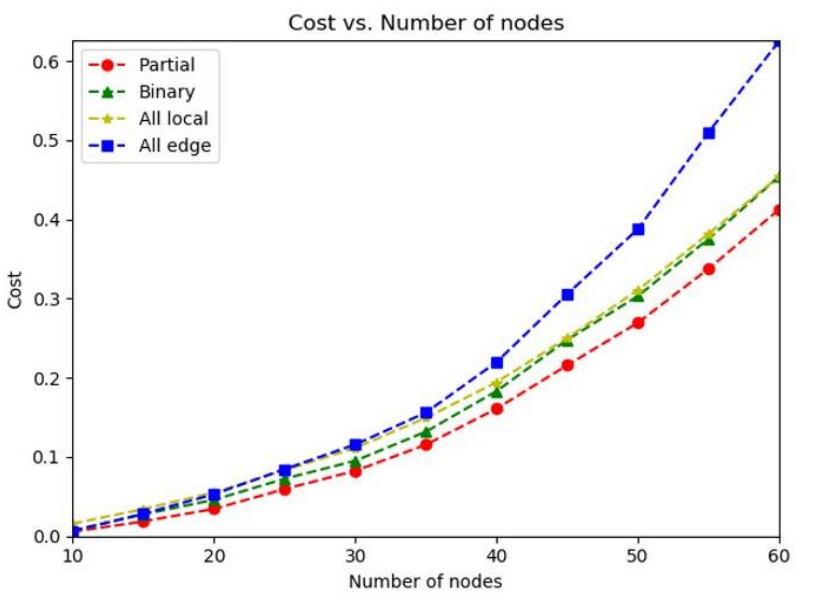
\includegraphics[width=.45\textwidth]{images/1.png}
    \caption{Aggregated computing cost when data size is $10 Mbits$} \label{fig:1}
\end{figure}
\begin{figure}
    \centering
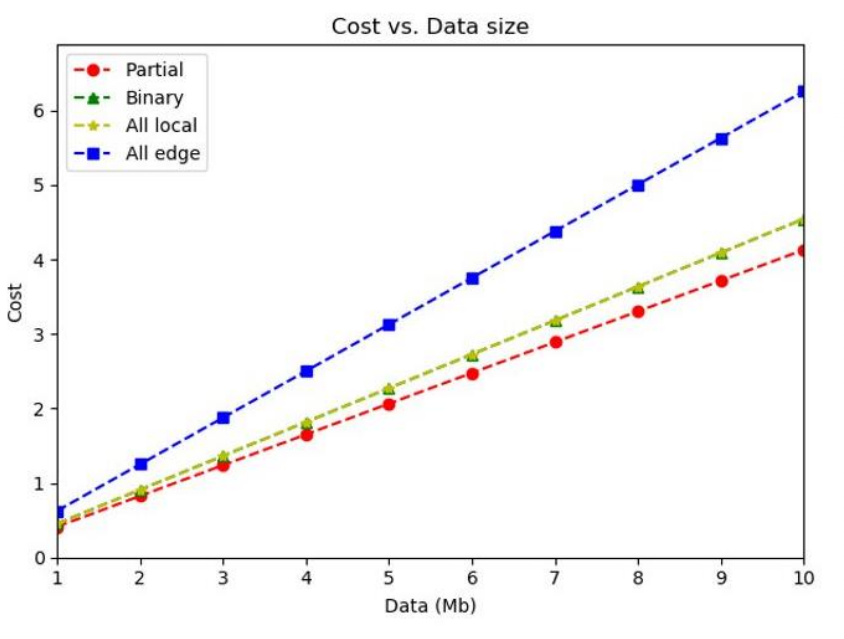
\includegraphics[width=.45\textwidth]{images/2.png}
\caption{Aggregated computing cost when we have $40$ nodes}\label{fig:2}
\end{figure}
\begin{figure}
    \centering
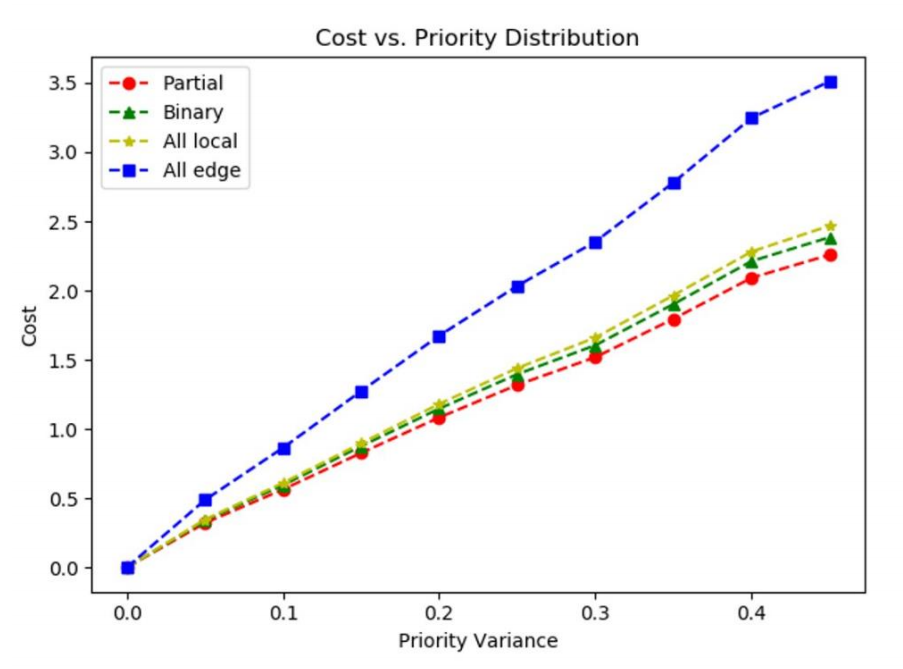
\includegraphics[width=.45\textwidth]{images/3.png}
\caption{Comparing aggregated computing cost for different priority variance}\label{fig:2}
\end{figure}

\begin{figure}
    \centering
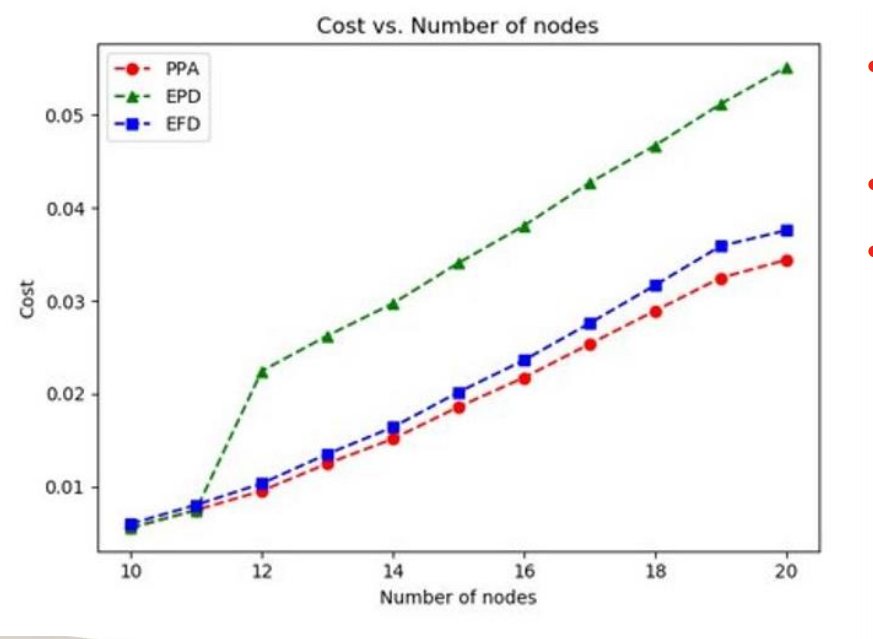
\includegraphics[width=.45\textwidth]{images/4.png}
\caption{Comparision between different peroposed methods}\label{fig:2}
\end{figure}


\bibliography{bibfile.bib} 
\bibliographystyle{ieeetr}

\end{document}



